%# -*- coding:utf-8 -*-
% Data Marketplace Agent Simulation — Beamer Presentation
% Based on ZJU Beamer Template

\PassOptionsToPackage{quiet}{fontspec}
\PassOptionsToPackage{dvipsnames}{xcolor}
\documentclass[10pt,aspectratio=169]{beamer}
\usepackage{zju_beamer}
\usepackage{booktabs}
\usetikzlibrary{positioning}
\graphicspath{{./figures/}}

\zjusectioncolor{blue}

% ============================================================
% 首页信息
% ============================================================
\title[数据市场 Agent 模拟]{基于 Agent 的数据市场机制模拟与改进}
\subtitle{：A Marketplace for Data: An Algorithmic Solution}
\author[]{杨馨懿\ 郑伊霞\ 周首航}
\date{\today}

\begin{document}

% ============================================================
% 标题页
% ============================================================
\begin{frame}
	\titlepage
\end{frame}

% ============================================================
% 目录页
% ============================================================
\begin{frame}
	\frametitle{目录}
	\tableofcontents
\end{frame}

% ============================================================
% Section 1: 背景与机制设计
% ============================================================
\section{背景与机制设计}

% --- 总览 ---
\begin{frame}
	\frametitle{总览}

	\begin{center}
		\begin{tikzpicture}[node distance=0.5cm, auto,
			block/.style={rectangle, draw, rounded corners, text width=3.1cm, align=center, minimum height=1.4cm, font=\footnotesize},
			arrow/.style={->, >=stealth, thick, blue!60}]

			\node[block, fill=blue!5] (P1) {\textbf{问题}\\ML 训练数据交易\\现有市场机制不适用};
			\node[block, fill=green!5, right=0.15cm of P1] (P2) {\textbf{论文方案}\\Agarwal et al. (2019)\\四大算法机制};
			\node[block, fill=yellow!8, right=0.15cm of P2] (P3) {\textbf{基本假设}\\理性参与 + 私有估值\\+ 短视/单阶段博弈};
			\node[block, fill=orange!10, right=0.15cm of P3] (P4) {\textbf{我们的工作}\\LLM Agent 替代理性参与者\\发现问题 $\rightarrow$ 提出改进};

			\draw[arrow] (P1) -- (P2);
			\draw[arrow] (P2) -- (P3);
			\draw[arrow] (P3) -- (P4);
		\end{tikzpicture}
	\end{center}

\end{frame}

% --- 四个挑战 ---
\begin{frame}
	\frametitle{ML 训练数据为什么需要一个专门的交易市场}

	\begin{block}{ML 训练数据作为商品的四个独特挑战（Agarwal et al., 2019）}
		\begin{enumerate}
			\item \textbf{可无限复制}：零边际成本$\rightarrow$ 稀缺性定价模型直接失效
			\item \textbf{价值是组合性的}：一个数据集的价值取决于买方已有哪些其他数据$\rightarrow$ 无法独立定价
			\item \textbf{买方无法为单个数据集报价}：买方没有对特定数据集的先验价值判断
			\item \textbf{价值事前不可验证}：不先跑一遍 ML 任务，谁也不知道数据有没有用
		\end{enumerate}
	\end{block}

	\begin{alertblock}{关键}
		买方真正知道的不是``这个数据集值多少钱''，而是\textbf{``预测精度提升 1\% 对我来说值多少钱''}。\\
		因此市场的交易单位不应是``数据集''，而应是\textbf{预测精度的边际提升}。
	\end{alertblock}
\end{frame}

% --- 市场架构 ---
\begin{frame}
	\frametitle{论文提出的机制}

	\begin{columns}[T]
		\begin{column}{0.38\textwidth}
			\begin{block}{三方参与者}
				\begin{itemize}
					\item \textbf{平台}：中心化定价，运行 ML 模型，结算分成
					\item \textbf{买家}：提交预测任务 $Y_n$ 和报价 $b_n$
					\item \textbf{卖家}：提供数据特征 $X_j$，被动接受分成
				\end{itemize}
			\end{block}
			\vspace{0.3cm}
			\begin{center}
				\small\textbf{买方不接触原始数据，只拿到模型预测结果}
			\end{center}
		\end{column}
		\begin{column}{0.60\textwidth}
			\begin{block}{单轮交易}
				\begin{enumerate}
					\small
					\item 买家提交预测任务 $Y_n$
					\item 买家报价 $b_n$（\textit{``精度提升 1\% 付 \$X''}）
					\item AF 分配数据：$b_n \ge p_n$ 给完整数据，否则加噪声
					\item 平台训练 ML 模型，计算精度增益 $G(Y_n, \hat{Y}_n)$
					\item RF（Myerson）计算支付额：\textbf{诚实报价占优}
					\item PD（Shapley）分配收入给卖家：\textbf{复制者受罚}
					\item PF（MWU）更新下一轮价格：\textbf{无遗憾定价}
				\end{enumerate}
			\end{block}
		\end{column}
	\end{columns}
\end{frame}

% --- 四大机制及其设计理由 ---
\begin{frame}
	\frametitle{四大机制及其设计理由}

	\begin{center}
		\footnotesize
		\renewcommand{\arraystretch}{1.6}
		\begin{tabular}{p{2.2cm}|p{2.8cm}|p{7cm}}
			\toprule
			\textbf{机制} & \textbf{应对的挑战} & \textbf{设计逻辑} \\
			\midrule
			AF（数据分配） & 事前不可验证 & 买方不接触原始数据：平台统一训练模型输出预测，避免数据泄露 \\
			\midrule
			RF（Myerson 支付） & 策略性谎报 & Myerson 支付函数数学上保证 $b_n = \mu_n$ 是占优策略：诚实报价收益最高 \\
			\midrule
			PF（MWU 定价） & 最优价格未知 & MWU 在候选价格网格上实现 no-regret：价格自动收敛至最优 \\
			\midrule
			PD（Shapley 分配） & 可复制 + 组合价值 & Shapley 值衡量边际贡献；余弦相似度指数惩罚复制数据 \\
			\bottomrule
		\end{tabular}
	\end{center}

\end{frame}

% --- 仿真截图 ---
\begin{frame}
	\frametitle{机制仿真：理论结果复现}

	\begin{center}
		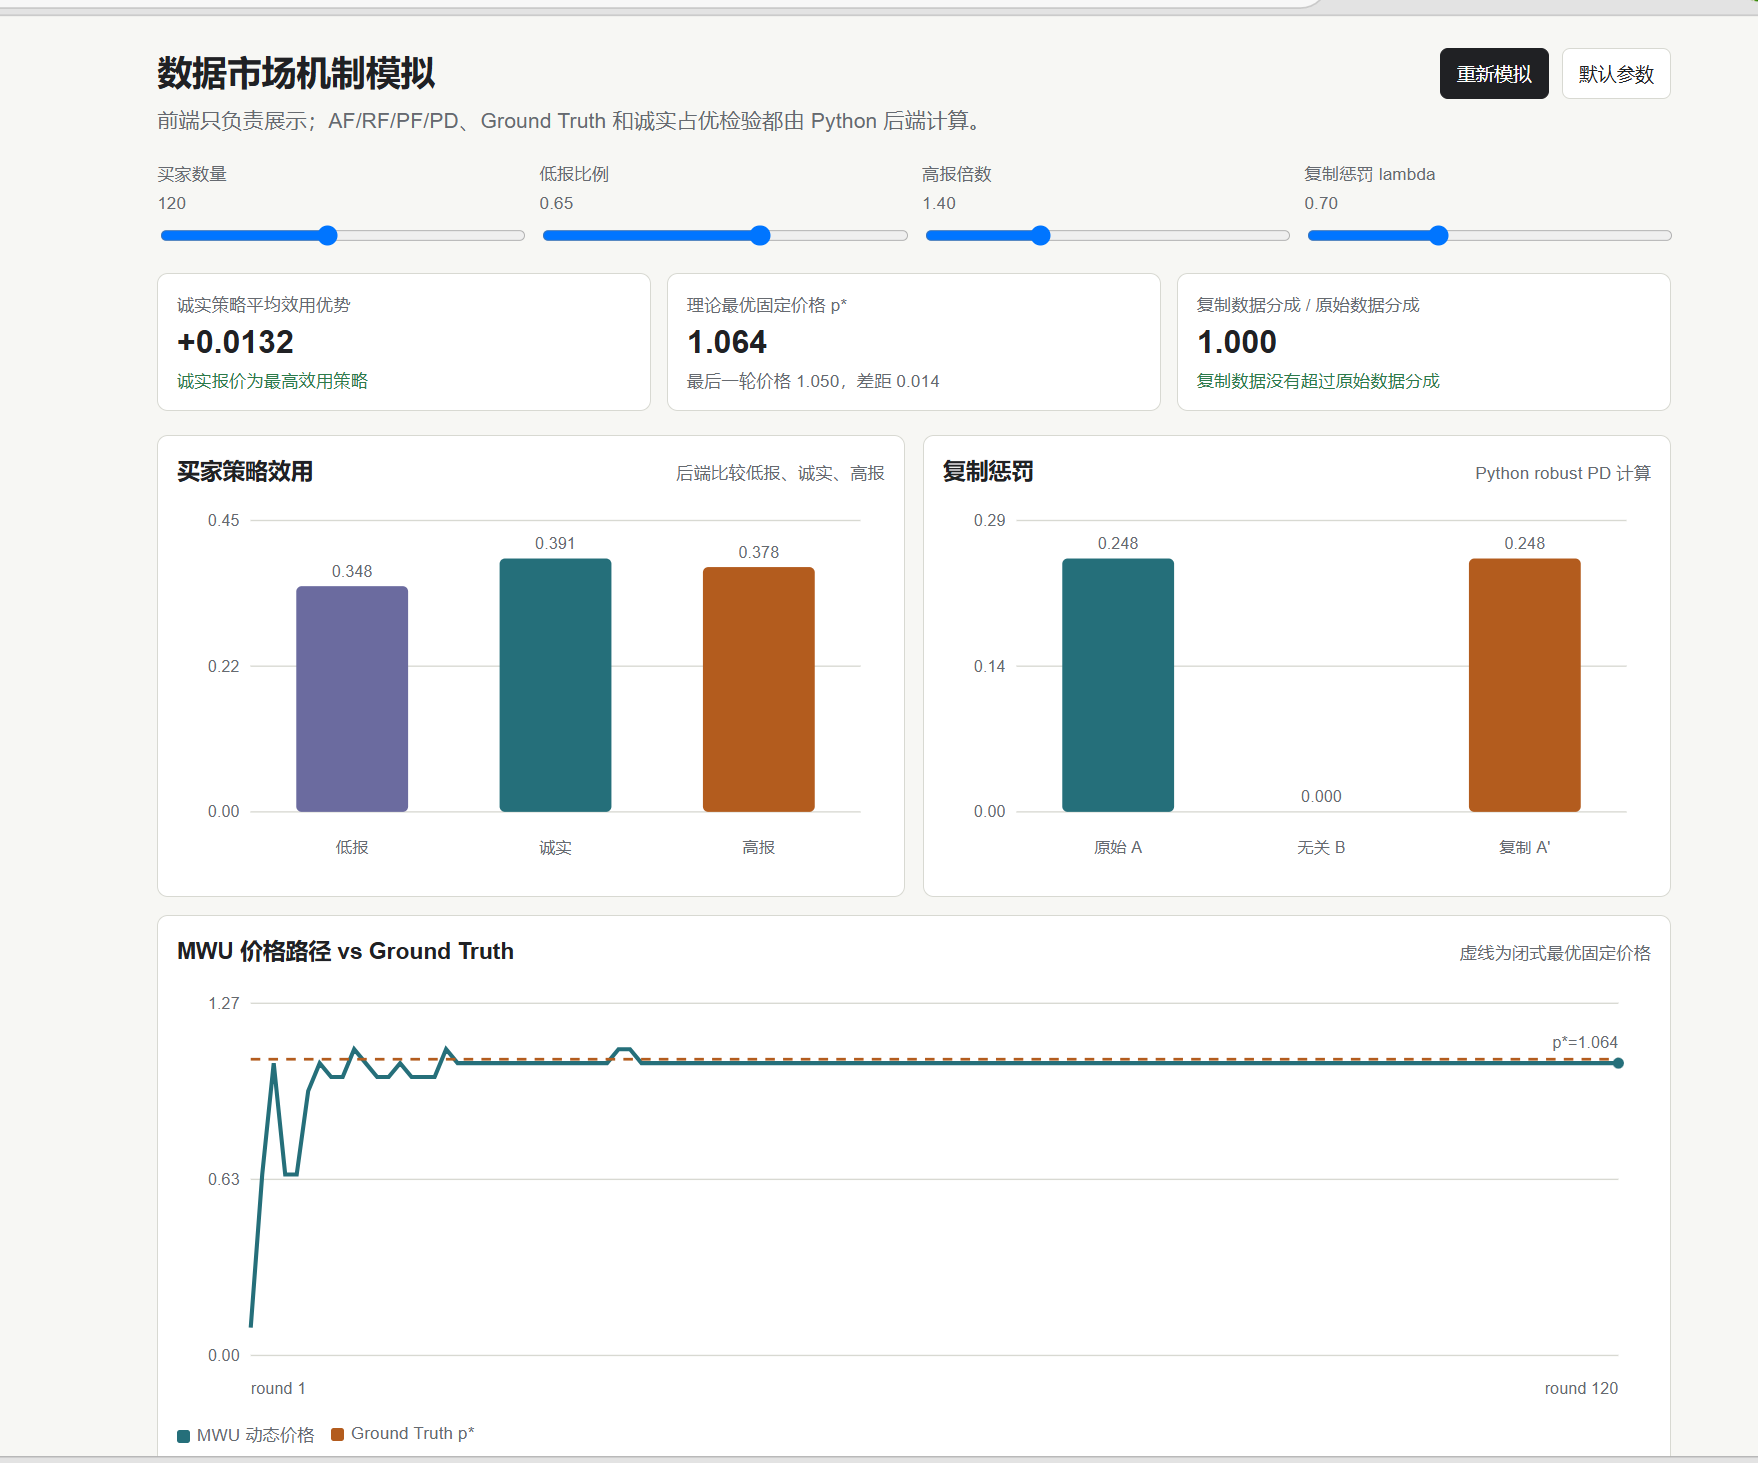
\includegraphics[height=0.68\textheight,keepaspectratio]{simulation.png}
	\end{center}

	\vspace{0.1cm}
	{\small 基于 AF / RF / PF / PD 机制实现，验证诚实报价占优、MWU 价格收敛、复制惩罚三项理论性质}
\end{frame}

% --- 论文自身的局限性 ---

\begin{frame}
	\frametitle{该机制的局限性}

	\begin{block}{局限}
		\begin{enumerate}
			\item \textbf{买家是短视的}：只优化单轮效用，不考虑多轮策略
			\item \textbf{买家效用仅来自预测质量}：而非来自特定数据集本身
			\item \textbf{平台集中定价}：卖家不能自主定价，只能被动接受 Shapley 分成
			\item \textbf{基于严格的私有估值假设}：忽视了数据的竞争外部性（买家效用往往受对手是否获取数据的影响）
			\item \textbf{卖家完全被动}：不能提高数据质量、不了解预测任务、不关心隐私
		\end{enumerate}
	\end{block}

	\vspace{0.2cm}
	\begin{center}
		\textbf{论文假定买家为理性、短视的私有估值者，诚实报价仅作为其在单阶段博弈下的占优策略}\\
	\end{center}
\end{frame}

% ============================================================
% Section 2: 我们的方法
% ============================================================
\section{我们的方法}

\begin{frame}
	\frametitle{用 LLM Agent 模拟真实市场参与者}

	\begin{block}{核心思路}
		保持论文的\textbf{市场机制完全不变}（AF / RF / PF / PD 照原样实现），\\
		把规则化的买卖双方替换为 \textbf{LLM Agent}，观察行为偏差。
	\end{block}

	\begin{columns}[T]
		\begin{column}{0.48\textwidth}
			\begin{exampleblock}{买家 Agent（LLM）}
				\textbf{看到}：当前价格 $p_n$、数据描述、历史成交、自己的估值 $\mu_n$、预算\\
				\textbf{决策}：报价 $b_n$ + 决策理由\\
				\textbf{研究}：Agent 会诚实报价吗？什么因素导致偏离？
			\end{exampleblock}
		\end{column}
		\begin{column}{0.48\textwidth}
			\begin{exampleblock}{卖家 Agent（LLM）}
				\textbf{看到}：自己的数据特征、历史分成、市场行情\\
				\textbf{决策}：是否复制数据、是否调整数据质量\\
				\textbf{研究}：Shapley 惩罚能否阻止 Agent 的复制行为？
			\end{exampleblock}
		\end{column}
	\end{columns}

	\pause
	\vspace{0.3cm}
	\begin{center}
		\textbf{对比实验}：理论最优vs.\ LLM Agent $\rightarrow$ 测量行为偏差 $\rightarrow$ 提出机制改进
	\end{center}
\end{frame}

\begin{frame}
	\frametitle{核心研究问题}

	\begin{enumerate}
		\item \textbf{LLM Agent 的诚实性}
		      \begin{itemize}
			      \item 面对 Myerson 支付规则，LLM Agent 是否会自发学会诚实报价？
			      \item 诚实报价 vs.\ 策略性低报：Agent 选哪个？为什么？
		      \end{itemize}

		\pause
		\item \textbf{多轮博弈中的合谋行为}
		      \begin{itemize}
			      \item 多个买家 Agent 在反复交易中，是否会集体压低报价？
			      \item MWU 定价机制能否抵御这种隐性合谋导致的价格下行？
		      \end{itemize}

		\pause
		\item \textbf{机制的鲁棒性}
		      \begin{itemize}
			      \item 买卖双方都是 LLM Agent 博弈时，MWU 价格还会收敛吗？
			      \item Shapley 惩罚还能有效阻止复制行为吗？
		      \end{itemize}

		\pause
		\item \textbf{改进方向}
		      \begin{itemize}
			      \item 基于 Agent 的行为偏差，解释机制为什么有问题
			      \item 探索更贴近现实的合理市场机制设计
		      \end{itemize}
		
		\pause
		\item \textbf{私有估值假设与竞争外部性}
		      \begin{itemize}
			      \item 当引入商业竞争（对手购买同一数据）时，Agent 的估值是否会发生动态耦合？
			      \item 在存在竞争外部性（非私有估值）时，原本保证诚实的 Myerson 机制是否会面临失效？
		      \end{itemize}
	\end{enumerate}
\end{frame}

% ============================================================
% Section 3: Agent 设计 (待填写)
% ============================================================
\section{Agent 设计}

\begin{frame}
	\frametitle{Agent 设计}

	\begin{center}
		\vspace{2cm}
		{\Large \color{black!50}（待填写）}

		\vspace{1cm}
		\textit{--- 买家 Agent 的 Prompt 设计、决策空间、LLM 选型等 ---}
	\end{center}
\end{frame}

% ============================================================
% Section 4: 已完成的模拟内容 (待填写)
% ============================================================
\section{已完成的模拟内容}

\begin{frame}
	\frametitle{已完成的模拟内容}

	\begin{center}
		\vspace{2cm}
		{\Large \color{black!50}（待填写）}

		\vspace{1cm}
		\textit{--- 机制层实现、环境层搭建、基线实验结果等 ---}
	\end{center}
\end{frame}

% ============================================================
% Section 5: 后续计划 (待填写)
% ============================================================
\section{后续计划}

\begin{frame}
	\frametitle{后续计划}

	\begin{center}
		\vspace{2cm}
		{\Large \color{black!50}（待填写）}

		\vspace{1cm}
		\textit{--- LLM Agent 集成、信息披露实验、Trial 机制、论文撰写等 ---}

	\end{center}
\end{frame}

% ============================================================
% 参考文献
% ============================================================
\section{参考文献}

\begin{frame}[allowframebreaks]
	\frametitle{参考文献}

	\begin{thebibliography}{10}

		\bibitem{agarwal2019}
		Anish Agarwal, Munther Dahleh, and Tuhin Sarkar.
		\newblock A Marketplace for Data: An Algorithmic Solution.
		\newblock In \textit{Proceedings of the 2019 ACM Conference on Economics and Computation (EC '19)}, 2019.

						\bibitem{wu2026}
		Wu P, Chen P Q, Li X, et al.
		\newblock Datamart-Agent: LLM-Driven Game-Theoretic Agent for Data Marketplace Modeling.
		\newblock In \textit{Findings of the Association for Computational Linguistics: ACL 2026}, 2026: 32509--32531.

\bibitem{li2024}
		Nian Li, Chen Gao, Mingyu Li, Yong Li, and Qingmin Liao.
		\newblock EconAgent: Large Language Model-Empowered Agents for Simulating Macroeconomic Activities.
		\newblock In \textit{Proceedings of ACL 2024}, 2024.


		\end{thebibliography}
\end{frame}

% ============================================================
% 结尾页
% ============================================================
\begin{frame}
	\frametitle{}
	\begin{center}
		\vspace{2cm}
		{\huge 谢谢！}
	\end{center}
\end{frame}

\end{document}
